\documentclass[12pt,a4paper,austrian]{article}
\usepackage{graphicx}
\usepackage[austrian, english]{babel}
\usepackage[utf8]{inputenc}
%\usepackage{listings}
\usepackage{multirow}
\usepackage{epstopdf}
\usepackage{amsmath}
\usepackage{amssymb} % fuer Mengen \N, Q, C, R
\usepackage{matlab-prettifier}
\graphicspath{{./fig/}}

\usepackage[colorlinks=true, pdfborder={0 0 0}, linkcolor=red]{hyperref}
\usepackage{float}


%% Satzspiegel
\setlength{\hoffset}{-1in} \setlength{\textwidth}{18cm}
\setlength{\oddsidemargin}{1.5cm}
\setlength{\evensidemargin}{1.5cm}
\setlength{\marginparsep}{0.7em}
\setlength{\marginparwidth}{0.5cm}

\setlength{\voffset}{-1.9in}
\setlength{\headheight}{12pt}
\setlength{\topmargin}{2.6cm}
   \addtolength{\topmargin}{-\headheight}
\setlength{\headsep}{3.5cm}
   \addtolength{\headsep}{-\topmargin}
   \addtolength{\headsep}{-\headheight}
\setlength{\textheight}{27cm}

%% How should floats be treated?
\setlength{\floatsep}{12 pt plus 0 pt minus 8 pt}
\setlength{\textfloatsep}{12 pt plus 0pt minus 8 pt}
\setlength{\intextsep}{12 pt plus 0pt minus 8 pt}

\tolerance2000
\emergencystretch20pt

%% Text appearence
% English text
\newcommand{\eg}[1]%
  {\selectlanguage{english}\textit{#1}\selectlanguage{austrian}}

\newcommand{\filename}[1]
  {\begin{small}\texttt{#1}\end{small}}

\newcommand\IFT{\unitlength1mm\begin{picture}(10,2) \put (1,1)
{\circle{1.7}} \put(2,1){\line(1,0){5}} \put(8,1)
{\circle*{1.7}}\end{picture}}
\newcommand\FT{\unitlength1mm\begin{picture}(10,2) \put (1,1)
{\circle*{1.7}} \put(2,1){\line(1,0){5}} \put(8,1)
{\circle{1.7}}\end{picture}}

% A box for multiple choice problems
\newcommand{\choicebox}{\fbox{\rule{0pt}{0.5ex}\rule{0.5ex}{0pt}}}

\newenvironment{wahrfalsch}%
  {\bigskip\par\noindent\makebox[1cm][c]{richtig}\hspace{3mm}\makebox[1cm][c]{falsch}
   \begin{list}%
   {\makebox[1cm][c]{\choicebox}\hspace{3mm}\makebox[1cm][c]{\choicebox}}%
   {\setlength{\labelwidth}{2.31 cm}\setlength{\labelsep}{3mm}
    \setlength{\leftmargin}{2.61 cm}\setlength{\listparindent}{0pt}
    \setlength{\itemindent}{0pt}}%
  }
  {\end{list}}

\newcounter{theaufgabe}\setcounter{theaufgabe}{1}
\newenvironment{aufgabe}[1]%
  {\bigskip\par\noindent\begin{nopagebreak}
   \textsf{\textbf{Exercise \arabic{theaufgabe}}}\quad
      \textsf{\textit{#1}}\\*[1ex]%
\stepcounter{theaufgabe}\hspace{2ex}\end{nopagebreak}}
  {\par\pagebreak[2]}

% Innerhalb der Aufgaben erfolgt die weitere Unterteilung mittels einer
% enumerate Umgebung, die allerdings a), b),... zaehlen soll.
\renewcommand{\labelenumi}{\alph{enumi})}
\renewcommand{\labelenumii}{\arabic{enumii})}

% A box to tick for everything which has to done
\newcommand{\abgabe}{\marginpar{$\Box$}}
% Margin paragraphs on the left side
\reversemarginpar

% Language for listings
%\lstset{language=Vhdl,
%  basicstyle=\small\tt,
 % keywordstyle=\tt\bf,
 % commentstyle=\sl}

% No indention
\setlength{\parindent}{0.0cm}
% Don't number sections
\setcounter{secnumdepth}{0}

% prints a predefined preamble
% done this so that we don't have all the code later in the file
\newcommand{\printpreamble}{
  \pagestyle{plain}
  \thispagestyle{empty}
  \noindent
  \begin{minipage}[b][4cm]{1.0\textwidth}  
  \begin{center}
  \begin{bf} 
  \begin{large} Digital Signal Processing SS 2024 -- Exercise~3\end{large} \\
  \vspace{0.3cm}
  \begin{Large} Digital Signal Processing Tutorial  \end{Large} \\
  \vspace{0.3cm}
  \end{bf}
  \begin{large} 
  Group 23\\
  Aaron Zettler, 12105021\\
  Pascal Pilz, 12111234\\
  \end{large} 
  \end{center}
  \end{minipage}
  
  \noindent \rule[0.8em]{\textwidth}{0.12mm}\\[-0.5em]
}

%% Beginning of the text
%=======================================================================================

\begin{document}
\printpreamble

\begin{aufgabe}{} % Exercise 1 ---------------------------------------------------------
We have the analog signal
$$
x(t) = x_1(t) + x_2(t) = \sin{(2 \pi f_1 t)} + \sin{(2 \pi f_2 t)}
$$
with $f_1 = 4 \text{kHz}$ and $f_2 = 6\text{kHz}$. The signal is sampled with a sampling frequency of $f_s = 10\text{kHz}$.
  \begin{enumerate}
    \item In Figure~\ref{fig:1a} we draw the spectrum of $x(t)$. This was derived analytically by observing that $x(t)$ is composed of two separate sinusoidal signals.
    \begin{center}
      \begin{figure}[H]
        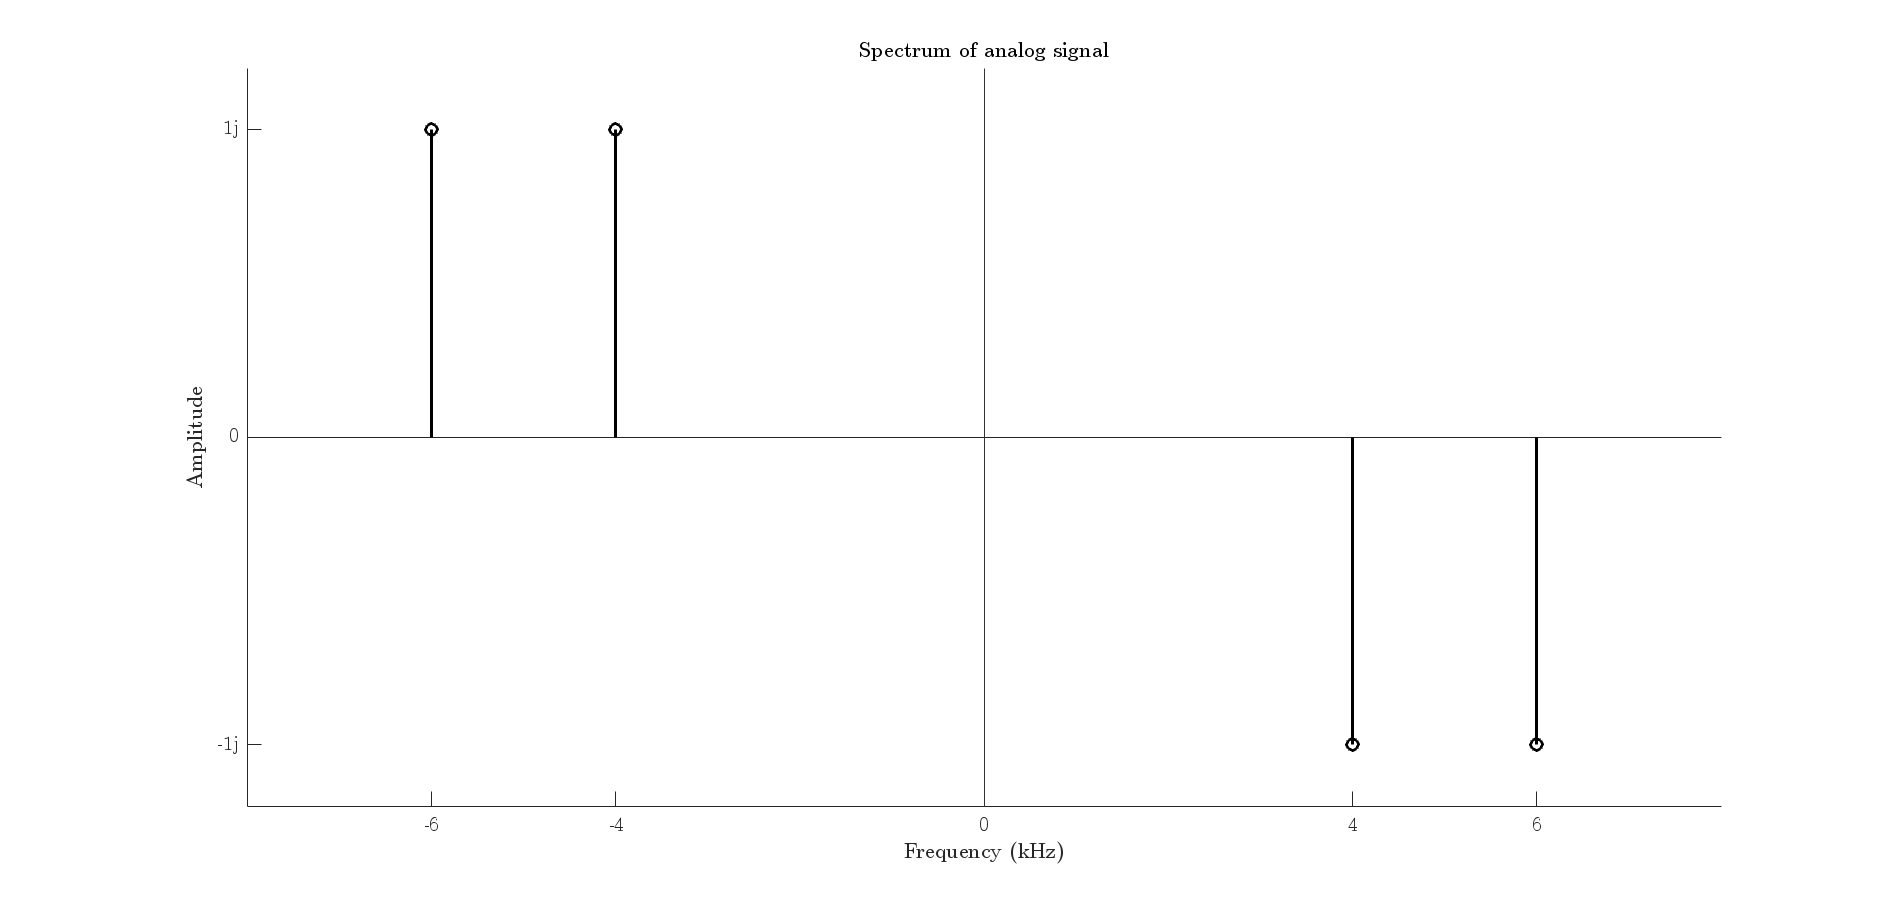
\includegraphics[width=0.9\textwidth]{../Ex01_a}
        \label{fig:1a}
        \caption{Spectrum of $x(t)$}
      \end{figure}
    \end{center}

    \item In Figure~\ref{fig:1b} we draw the spectrum of $x(t)$ shifted by $-f_s$, $0$, and $+f_s$, as well as the result of adding up the shifted spectra.
    \begin{center}
      \begin{figure}[H]
        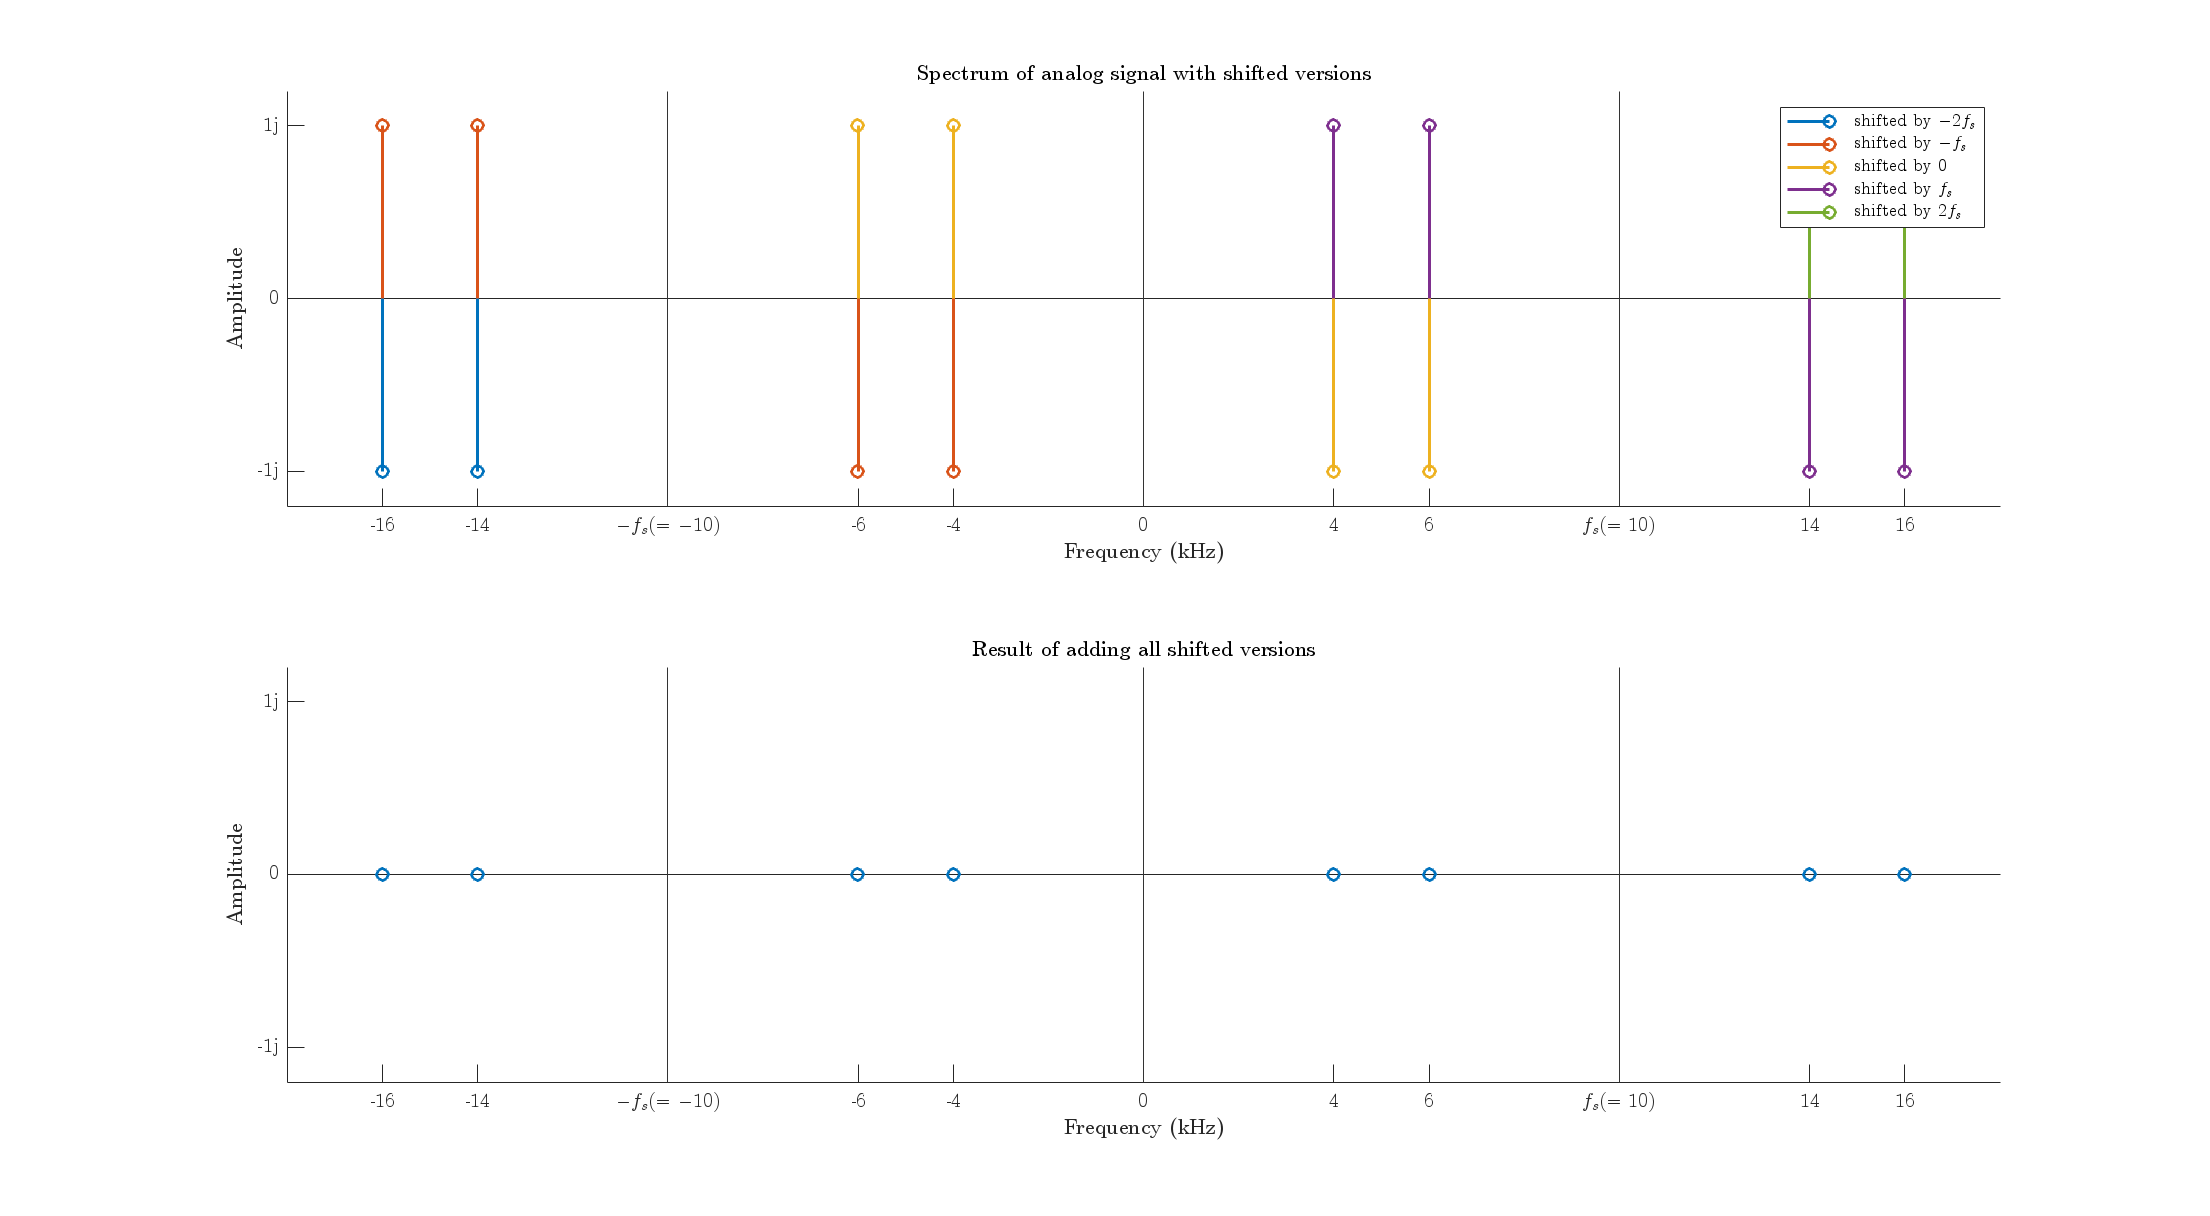
\includegraphics[width=0.9\textwidth]{../Ex01_b}
        \label{fig:1b}
        \caption{Spectrum of $x(t)$ shifted}
      \end{figure}
    \end{center}

    \item In Figure~\ref{fig:1c} we draw the first 2ms of the signal $x(t)$ and the resulting signal after sampling with $f_s = 10\text{kHz}$. As we can see, $x[t] = 0$, and therefore the spectrum will also be constant $0$.
    \begin{center}
      \begin{figure}[H]
        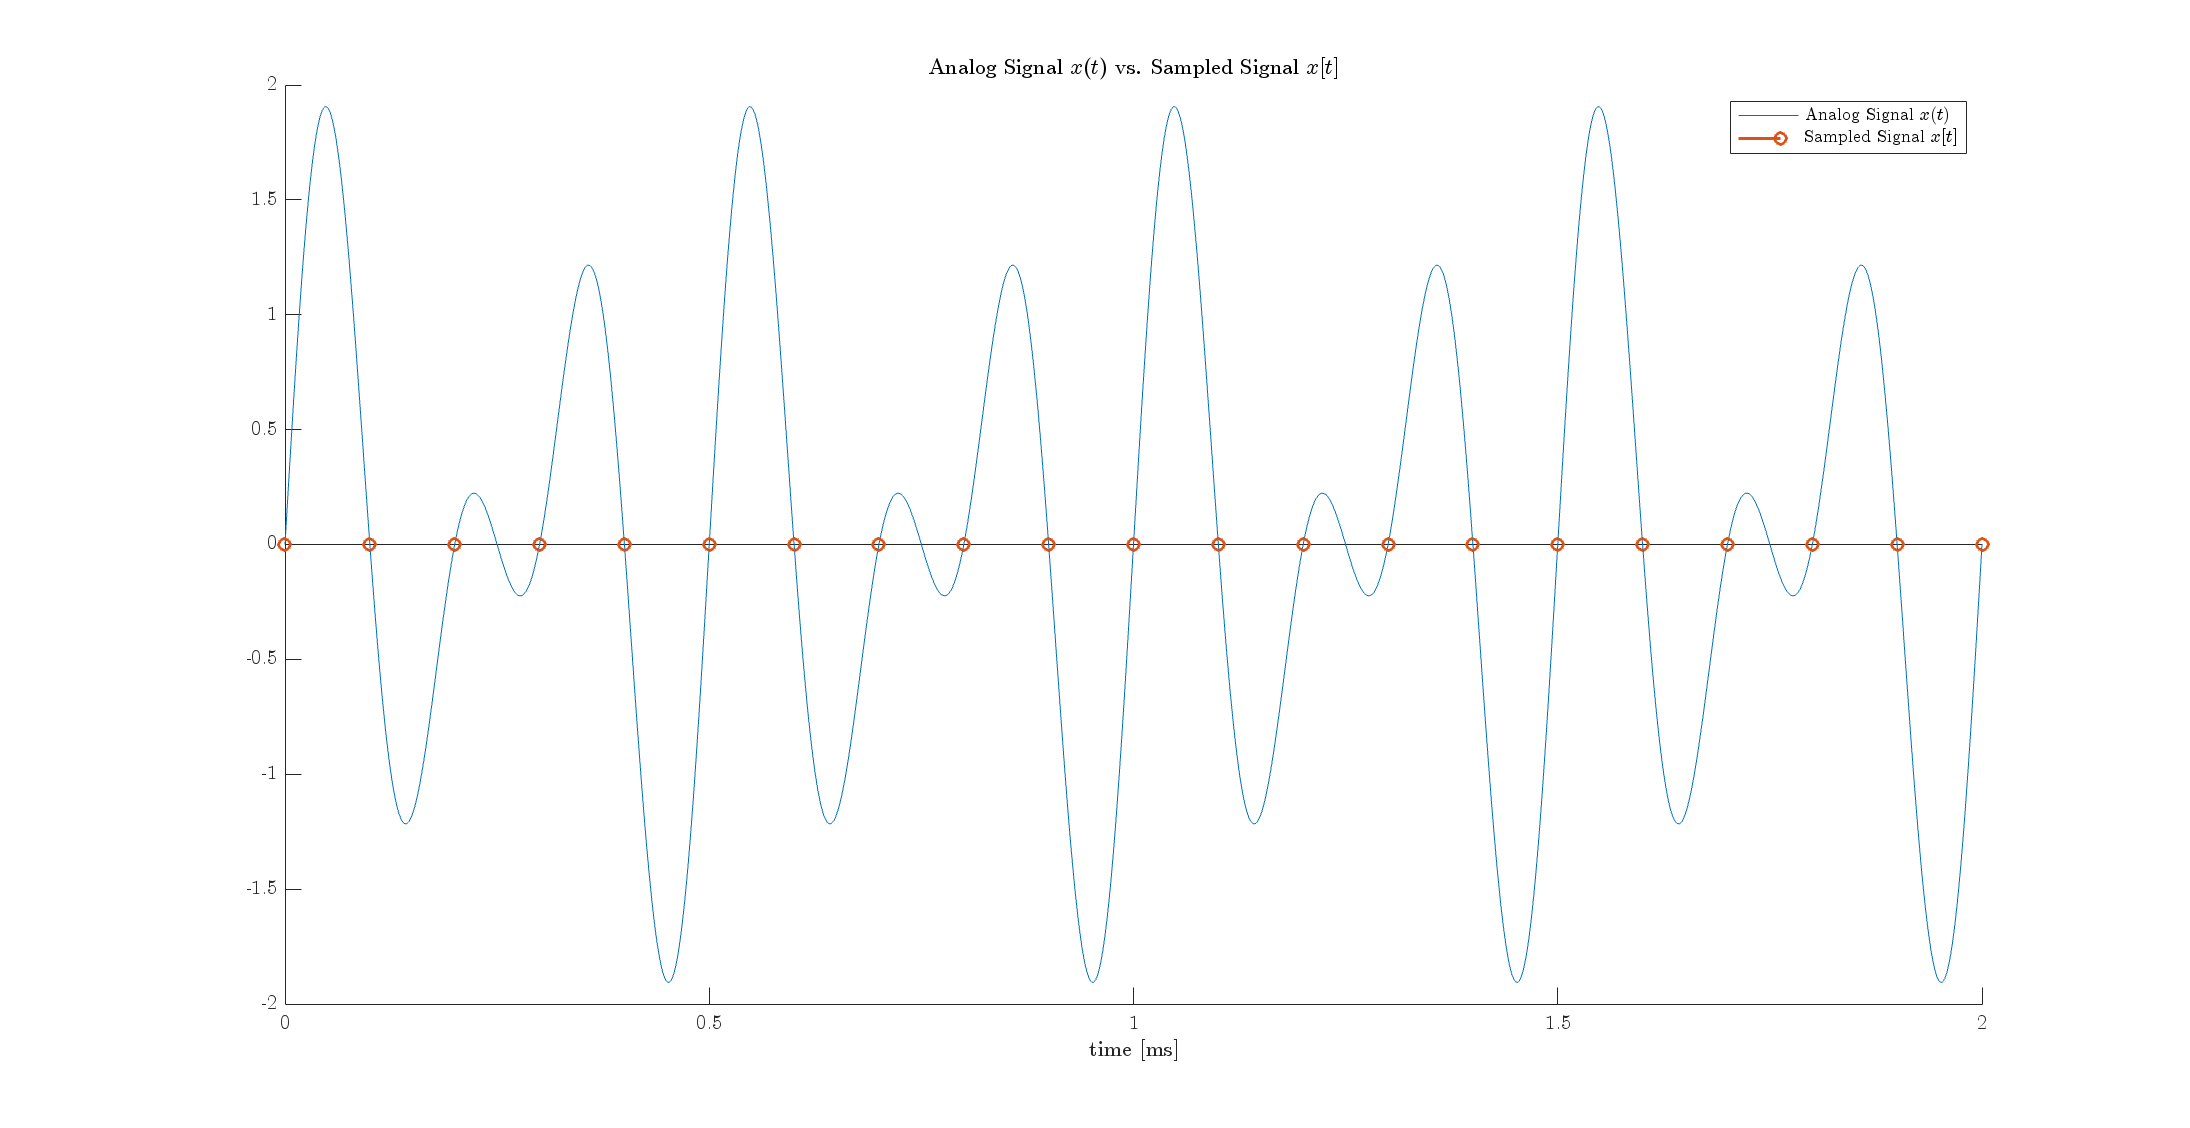
\includegraphics[width=0.9\textwidth]{../Ex01_c}
        \label{fig:1c}
        \caption{$x(t)$ and $x[t]$}
      \end{figure}
    \end{center}
  \end{enumerate}
\end{aufgabe} \pagebreak

\begin{aufgabe}{} % Exercise 2 ---------------------------------------------------------

\end{aufgabe} \pagebreak

\begin{aufgabe}{} % Exercise 3 ---------------------------------------------------------

\end{aufgabe} \pagebreak

\begin{aufgabe}{} % Exercise 4 ---------------------------------------------------------

\end{aufgabe} \pagebreak

\end{document}
